\chapter{Interaction design}
\chlab{design}

Here will be the interaction designs for the tool\ldots

\nlipsum


\section{Platform}
The requirements of the molecule parameterisation tool have been specified in \chref{problems}. It has been decided to implement the tool in \verb|HTML5| and \verb|JavaScript|, which allows for great portability and availability across different operating systems and platforms. It also makes the tool future-proof, by following the current trend of bringing everything to the web~\cite{ertl2010molecular}, examples of which are \verb|JSMol|~\cite{hanson2013jsmol} and \verb|JSME|~\cite{bienfait2013jsme}~(see also \secref{software}).

Not surprisingly, there are no existing tools for fragment-based molecule parameterisation, as this is a new concept. Furthermore, no tools exist for comparing molecules - or fragments of them - either. What does exist is a wide range of tools and programs for showing and editing molecules. This includes stand-alone molecule drawing software such as \verb|Accelerys Draw|~\cite{accelrys2012accelrys} and \verb|Avogadro|~\cite{hanwell2012avogadro}, two-dimensional web-based molecule editors like \verb|ChemDoodle 2D Sketcher|~\cite{ichemlabs2013chemdoodle}, \verb|Molsoft HTML5 Molecule Editor|~\cite{molsoft2012molsoft} and \verb|Marvin for JavaScript|~\cite{chemxon2013marvin}, and online three-dimensional visualisation tools \verb|JSMol|~\cite{hanson2013jsmol} and \verb|CanvasMol|~\cite{altered2013canvasmol}.

These existing tools will serve as an initial guideline for the tool to be developed, and parts of their implementations may be reused. The rest of the tool, however, will need to be designed and developed from scratch. The design will follow the basic interaction design principles as posed by Norman and others~(see \secref{id_principles}), the knowledge about learing~(see \secref{id_learning}), and keep in mind the insights gained by the developers of other molecule software~(see \secref{software}).


\section{Two versions}
As there is no existing software for fragment-based molecule parameterisation, there is also no baseline to which the developed tool can be compared. In order to still be able to say something about the quality of the tool, two different implementations of it will be made. There are a few axles along which this difference can be made. One could, for instance, compare two tools that have different visualisation methods. Visualising molecules, however, is a well-exhausted field of research, leaving very little room for new ideas. Furthermore, molecules cannot be represented in textual form here, as a visual representation is essential to perceive similarity of fragments~\cite{gallopoulos1994computer}.

Another possible variable in the tool is the way its users will interact with it and especially its degree of automation. Varying this degree has been the subject of several studies~(e.g.~\cite{payne2000varying, horvitz1999principles, marcus1987taking, norman1990problem}, see also \secref{id_automation}), all of which concluded the degree to which automation can be applied is highly dependent on the context of the system and sometimes even to the situation in which the system is used.

When implementing multiple versions of a tool with different levels of interaction, it is often decided to make three versions: a `naive' version without much automation, a `cooperative' version in which the user is given advise, and an `autonomous' version that only requires some parameterisation~(see~\cite{payne2000varying} and \secref{id_automation}). As it is considered hard to parameterise a molecule based on fragments of other molecules and little is known on what is the best way of doing this, an autonomous version of a tool that does this cannot yet be developed. The other two versions, however, seem to be perfectly implementable and both can be considered useful.

\begin{figure}[h!]
\begin{center}
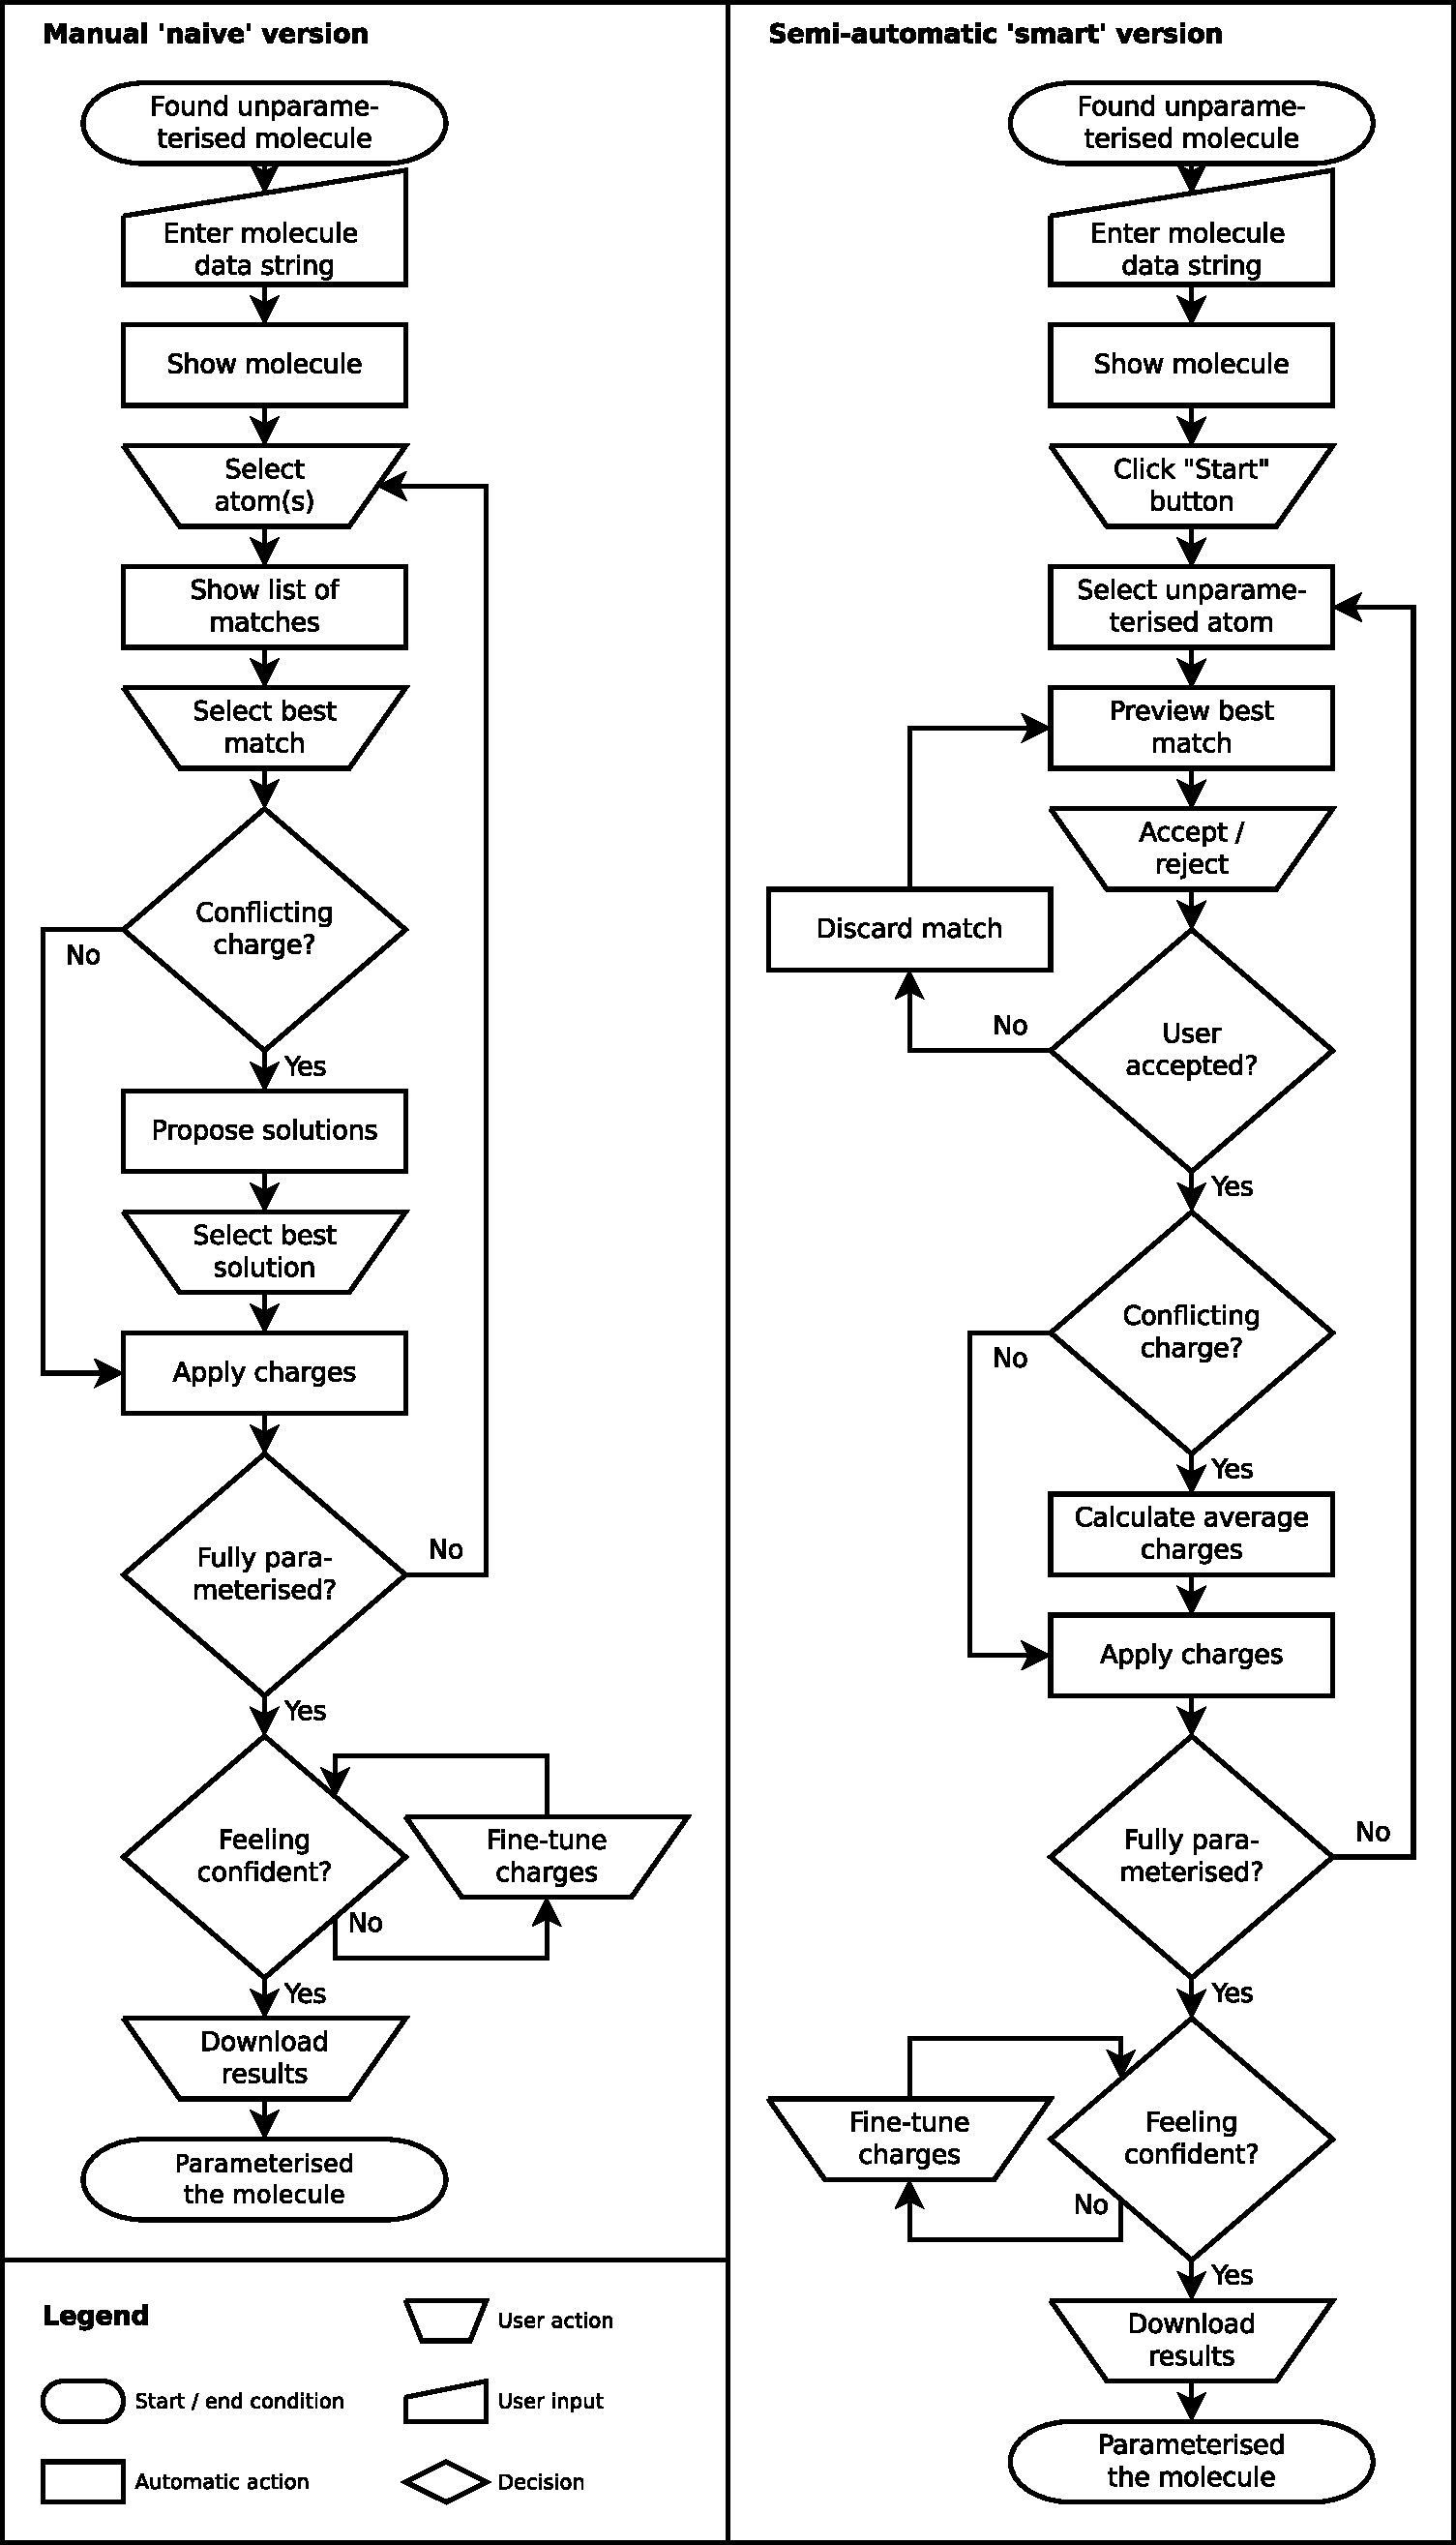
\includegraphics[width=.9\textwidth]{img/complete_id.pdf}
\caption{The two different interaction designs.}
\figlab{id_flows}
\end{center}
\end{figure}

\Figref{id_flows} shows a naive and a cooperative interaction design for the tool that will be developed. Here, the cooperative design has been called the `smart' version to accentuate its differences with the naive version. The following sections will discuss these two interaction designs, the motivation behind them, their workings, and the hypotheses about them.

\subsection{Manual `naive' version}
Just like the naive RPA implementation from~\cite{payne2000varying}, the naive version of the molecule parameterisation tool will only automatically perform user input validation. Besides ordering the matching fragments based on their probability of being a good match, the tool will not give any advise, nor will it automatically infer any values.

\subsubsection{Workings}
The complete set op steps required to fully parameterise a molecule using the naive version of the tool is as follows:
\begin{enumerate}[itemsep=.1em, parsep=.2em, topsep=0em]
\item The user enters a molecule data string (in \verb|SMILES|, \verb|InChI|, or other format). The molecule will be displayed to the user;
\item The user selects a single atom or a group of \emph{connected} atoms;
\item The user clicks the ``Find matches'' button;
\item A list of matching fragments will be shown, ordered such that the highest rated match comes first and the lowest last. The user can browse through them, preview the result of selecting that match and, once he has found what he sees as the best match, select this match. Hereafter, the charges from that match will be assigned to the molecule;
\item
\begin{itemize}[leftmargin=0cm, itemsep=.1em, parsep=.1em]
\item[]{\bf Unparameterised atoms remain}:\\The user selects another atom / list of connected atoms. Back to step 3;
\item[] {\bf Molecule fully parameterised}:\\Continue to step 6;
\end{itemize}
\item When needed, the user can fine-tune the atom charges by selecting an atom and modifying its charge using an input field. In order to assist him in this process, the fragments that were matched to this atom \emph{and} have been selected will be shown.
\end{enumerate}

\noindent
In the matching process, it is possible that an already charged atom is present in another chosen fragment. In the case where these charges differ, the user will be asked to decide what should happen, which can be one of:
\begin{enumerate}[itemsep=.1em, parsep=.2em, topsep=0em]
\item Take the average of the two charges;
\item Keep the current value;
\item Take the new value;
\item Manually enter a value.
\end{enumerate}

\subsubsection{Motivation}
As pointed out earlier, it is important to have a non-automatic baseline to see if automation can work for a certain tool. In this project, the naive version will serve as that baseline. However, it is more than just a baseline; it could also quite possibly work better than any automated version. The same was concluded for the naive RPA in~\cite{payne2000varying}, which was largely outperformed by its more automated siblings, but offered great benefits in situations where full control was required.

In the naive molecule parameterisation tool, the user can manually decide what atoms need to be parameterised and has a clear overview of all matching fragments. Furthermore, he can manually decide what should happen with overlapping fragments and can modify atom charges at any point in the process. This provides the same benefits as the previously discussed naive RPA had.

Another reason why this naive version might work better than an automated one is the fact that this one encourages exploring different options. By providing a list of fragments, rather than proposing a single one, the fragments can easily be compared such that the chances for the best match being selected increase. Furthermore, as the user is free to determine what atoms should be parameterised at which point in time and also to select groups of atoms, he can experiment with the selection size and order, which may lead to better results.


\subsection{Semi-automatic `smart' version}
Inspired on the cooperative RPA from~\cite{payne2000varying}, \verb|LookOut|~\cite{horvitz1999principles}, and \verb|SALT|~\cite{marcus1987taking}, the smart tool for molecule parameterisation continuously makes suggestions to the user. It will do so with possible matching fragments and atoms that might require fine-tuning, and will autonomously solve conflicting atom charges.

\subsubsection{Workings}
Using the semi-automatic version of the tool, the user should follow the following steps in order to fully parameterise a molecule:
\begin{enumerate}[itemsep=.1em, parsep=.2em, topsep=0em]
\item The user enters a molecule data string (in SMILES, InChI, or other format). The molecule will be displayed to the user;
\item The user clicks the ``Find matches'' button. One of the atoms will now be automatically selected and matching fragments will be retrieved;
\item The highest rated match is previewed on the molecule. The user can either accept or reject this proposed match;
\item
\begin{itemize}[leftmargin=0cm, itemsep=.1em, parsep=.1em]
\item[]{\bf Rejected}:\\Remove this match from the list of matching fragments (the user \emph{can} go back to this one if he changes his mind). Back to step 3;
\item[] {\bf Accepted}:\\Assign the charges of the fragment to the molecule. Continue to step 5;
\end{itemize}
\item
\begin{itemize}[leftmargin=0cm, itemsep=.1em, parsep=.1em]
\item[]{\bf Unparameterised atoms remain}:\\Another unparameterised atom is automatically selected and similar fragments are retrieved. Back to step 3;
\item[] {\bf Molecule fully parameterised}:\\Continue to step 6;
\end{itemize}
\item The user can now fine-tune the charges by selecting an atom and modifying the charge using some input field, if he wants to do so. In order to assist him in this process, suggestions will be given on what atoms to fine-tune and to what value they should be adjusted.
\end{enumerate}

\noindent
In the matching process, it is possible that an already charged atom is present in another chosen fragment. When these charges differ, the atom's charge will be automatically calculated from the two charges. Experimentation has yet to show the best way to do this, but, presumably, taking the average of the two will be a good solution.

\subsubsection{Motivation}
One of the most important reasons for developing a tool for fragment-based molecule parameterisation is to speed up the current process that uses quantum mechanical calculations. Having some automation in this tool can help increasing this benefits even further. By suggesting molecule fragments, parameterising a molecule can potentially be done a lot faster than when the user has to manually go through a list of fragments.

By automating certain parts of the parameterisation process, the tool should also be easier to use. One basically only needs to say `yes' or `no' a few times and will therefore be easy to learn. This increases the potential for new people to start using the tool, thereby enhancing its value. Furthermore, it makes sure users do not get lost in a long list of features. Otherwise, users might make the wrong decisions or even stop parameterising completely~\cite{norman2002design}~(see also \secref{design}).

In order to mediate the often occurring problems with automation, the fine-tuning step at the end has been added, based on studies by Norman~\cite{norman1990problem} and Horvitz~\cite{horvitz1999principles}. As there will always be errors in the automatic charge corrections, this provides the user with a way to identify and improve incorrectly assigned atom charges. The warnings that some atoms may be charged incorrectly will be non-intrusive, and the user will be able to see how every charge came to be in order to determine how to improve it.


\section{Interaction topology}
In order to be able to discuss visual interfaces at an abstract level, Brehmer and Munzner have developed a multi-level typology for abstract visualisation tasks~\cite{brehmer2013multi}~(see also \secref{id_abstraction}). The Brehmer-Munzner typology\footnote{It is not officially named, but will be referred to as the `Brehmer-Munzner typology' in the remainder of this document.} for the two implementations of the molecule parameterisation tool is shown in \figref{id_typologies}.

\begin{sidewaysfigure}[p]
\begin{center}
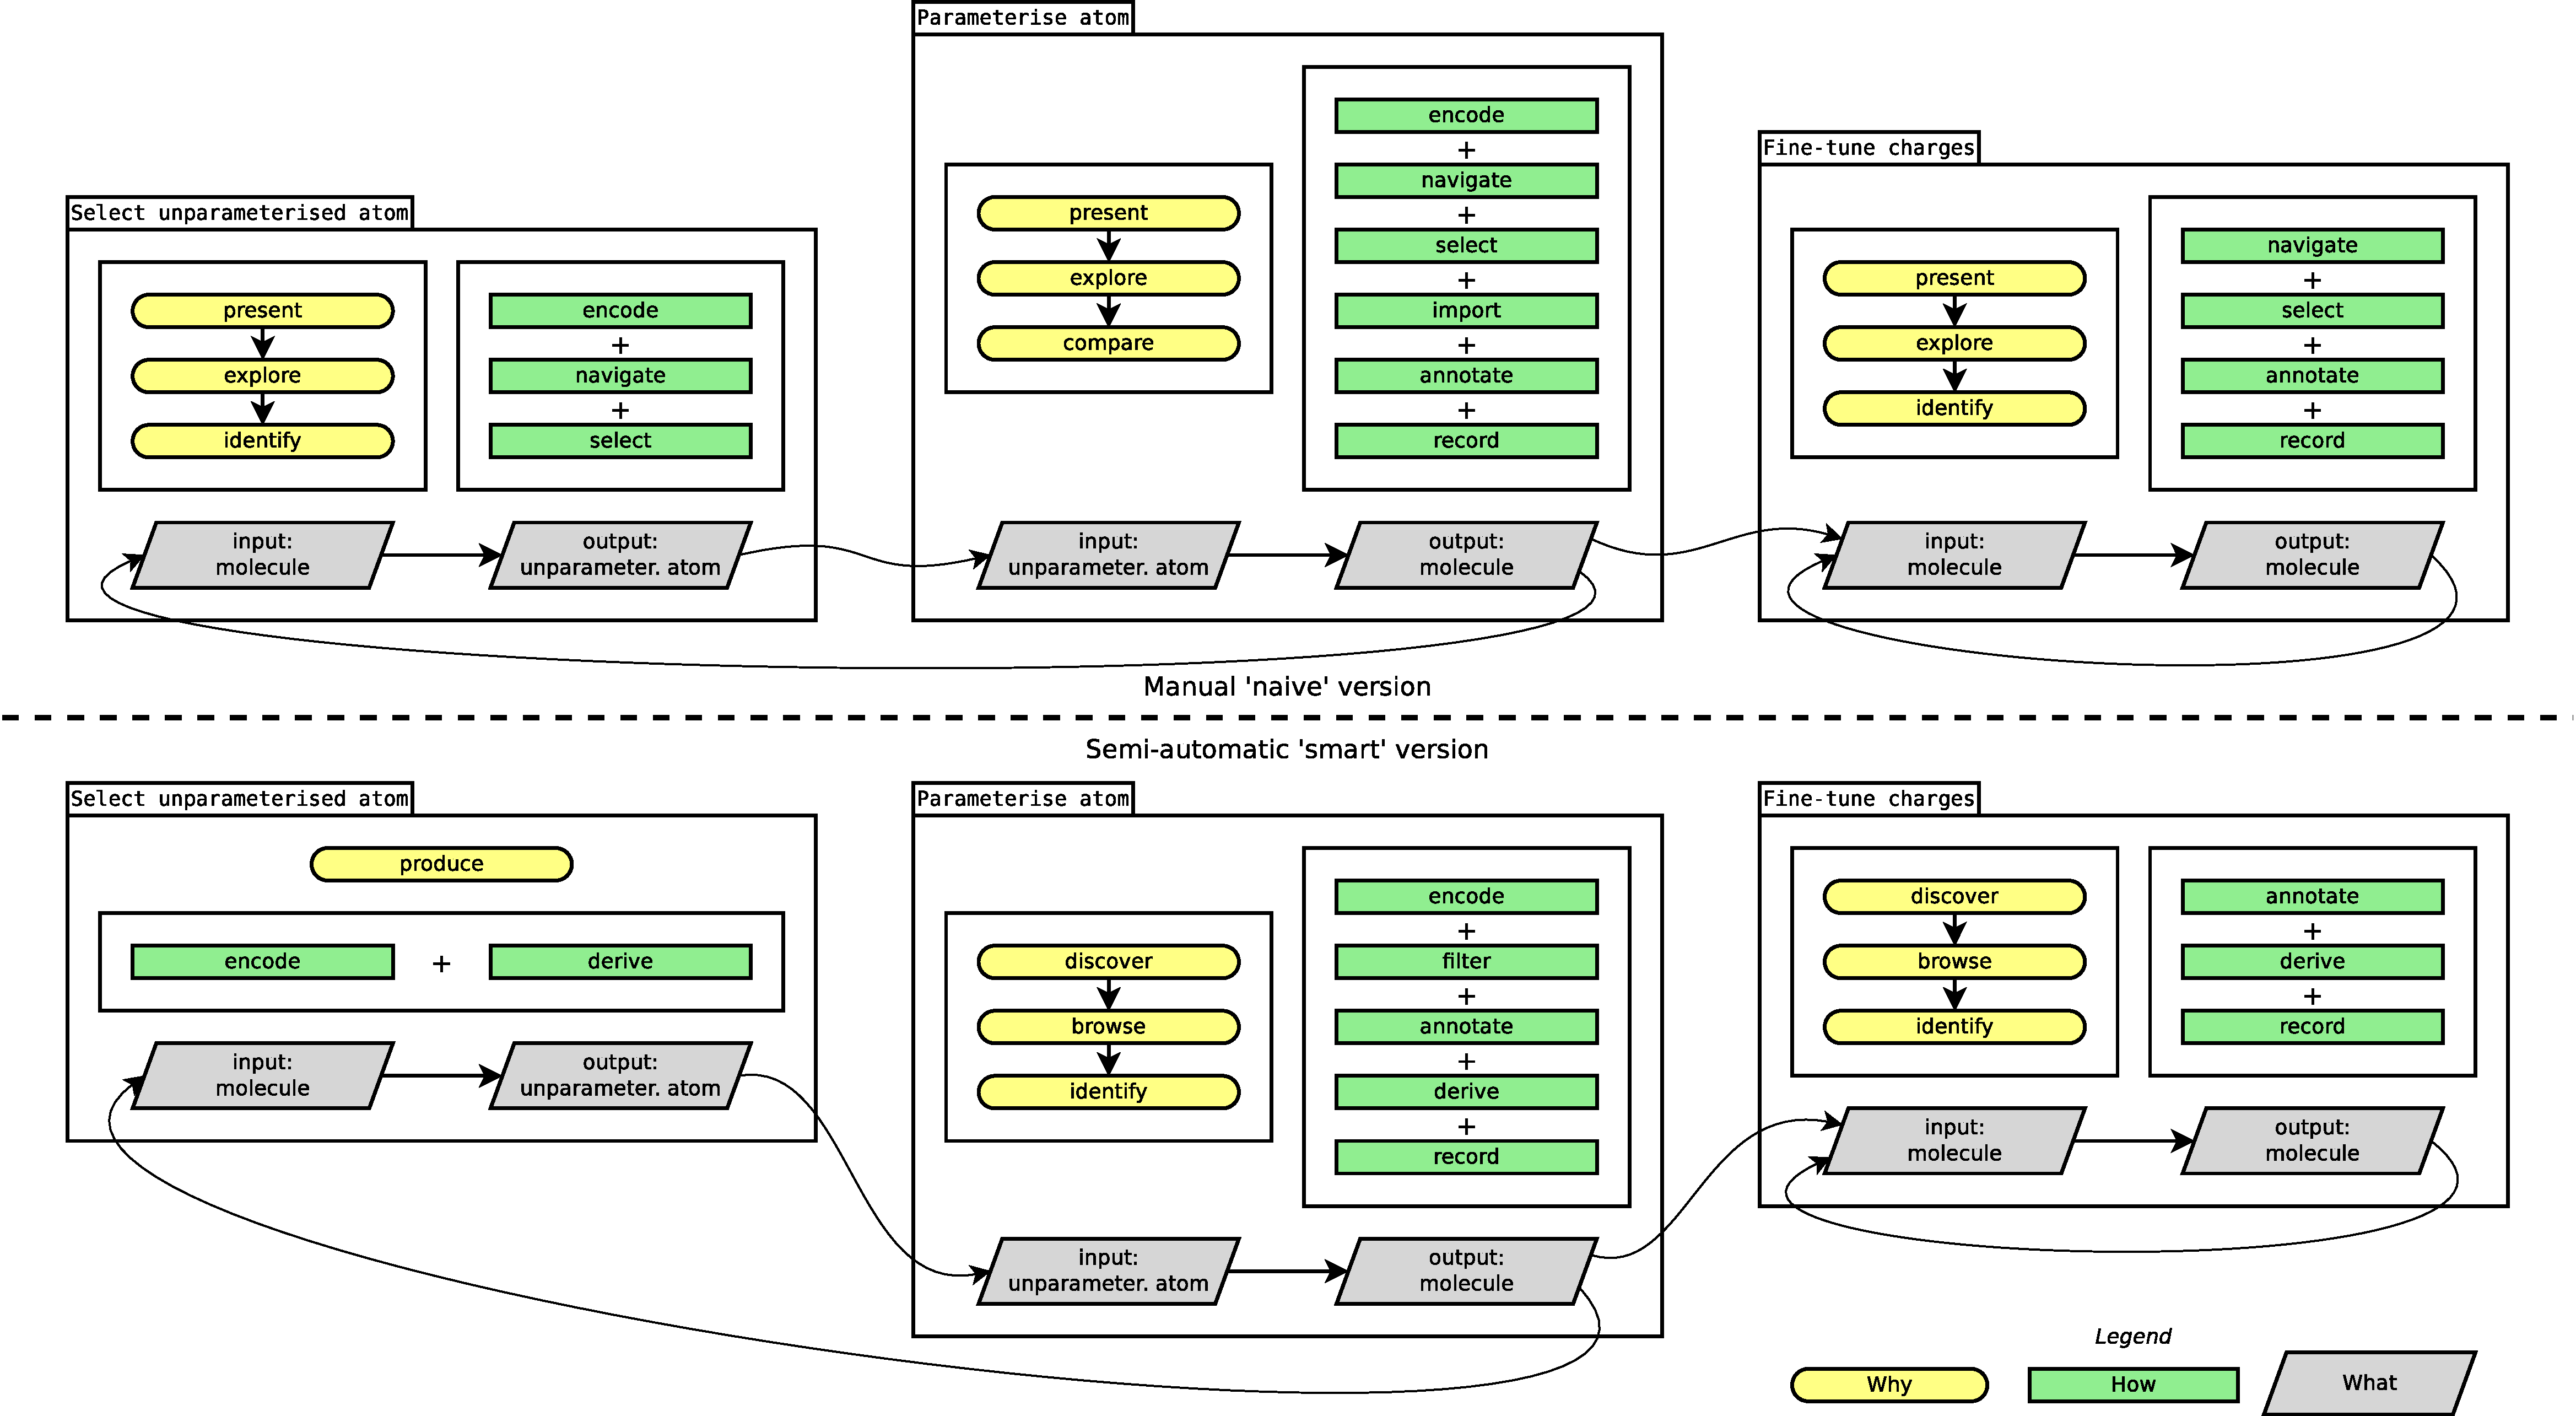
\includegraphics[width=\textwidth]{img/complete_typology.pdf}
\caption{Brehmer-Munzner Typologies of the two different interaction designs.}
\figlab{id_typologies}
\end{center}
\end{sidewaysfigure}

These typologies clearly outline the differences between the two implementations. While the naive version is mainly concerned with presenting things to the user and user exploration, in the smart version, the user is mainly discovering (verifying) the system's proposals and browsing through them. This means that, in the semi-automatic version, the user has easier access to the information, and can therefore make decisions earlier than in the naive version.

What is also clear in the typologies is the difference in the number of different methods that is required to parameterise a molecule in the two versions. In every step of the process, the smart version requires less different methods than the naive one. This does not necessarily mean that the smart version will take less time to use, as the methods may need to be used more often. What it does mean, however, is that it will be easier to use the smart version, as less different methods need to be used and learned~\cite{sweller1994cognitive}~(see also \secref{id_learning}).
